%
In 2001 the \gls{acr:peer} started a project aimed at validating
and comparing results provided by a number of public and private 
\gls{acr:psha} codes \parencite[for a comprehensive list see][]{thomas2010}.
%
For this purpose two set cases were created to check the way 
codes were implementing fundamental steps in the \gls{acr:psha}
calculation mechanics.
%
The major differences observed were appointed to differences in 
the numerical procedures adopted in the different software.
% 
The test acceptance level adopted corresponds to 10 percent in 
probability for a chosen value of ground motion intensity.
%
% ..............................................................................
\section{Test case set 1}
The test case set 1 was designed to test basic elements of the 
software such as \parencite{thomas2010}:
\begin{itemize}
\item modeling of ruptures on fault planes 
\item implementation of \glspl{acr:mfd}
\item modeling of area sources
\item modeling of ground motion variability
\end{itemize}
Figure \ref{fig:peer_sources} shows the geometry of the sources adopted 
in the first test case set. 
% . . . . . . . . . . . . . . . . . . . . . . . . . . . . . . . . . . . > Figure
\begin{figure}[!ht]
\centering
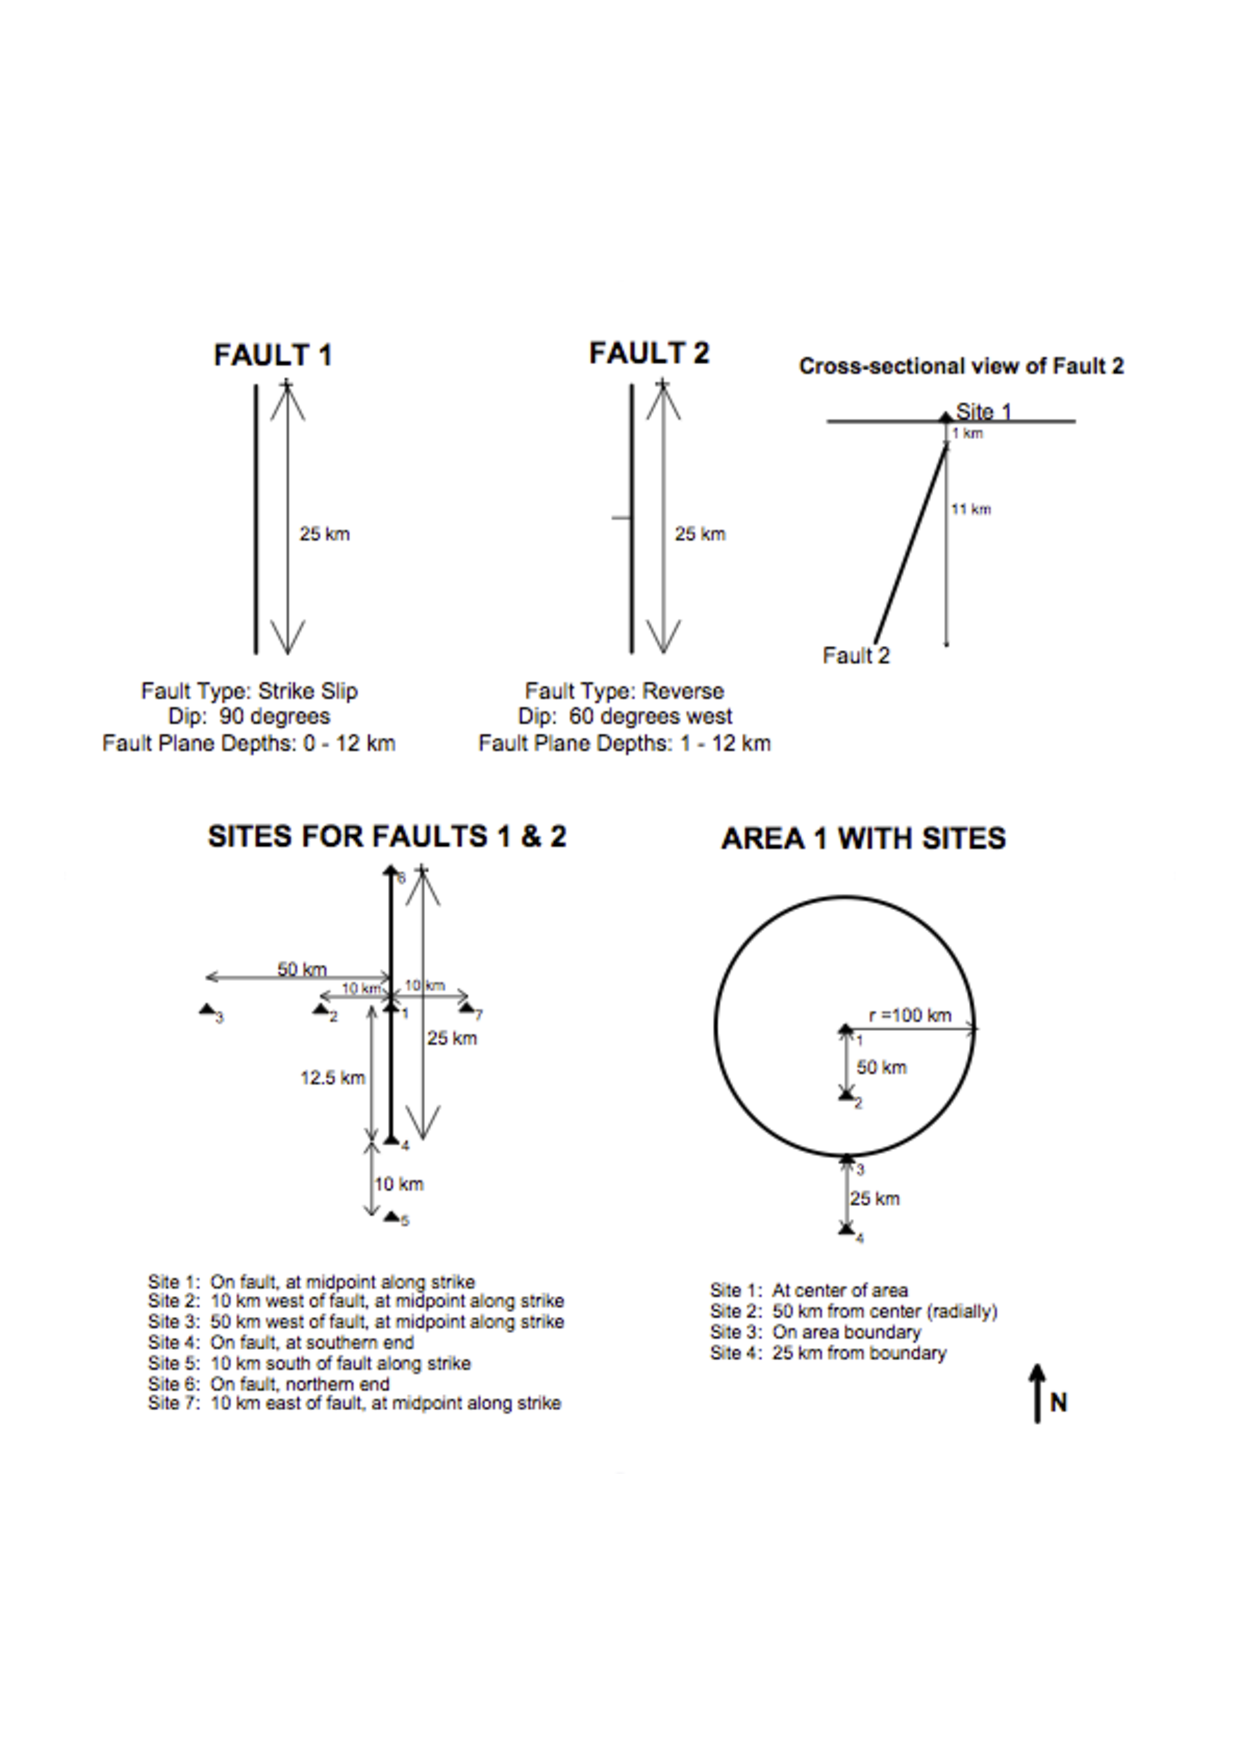
\includegraphics[trim=40mm 5mm 5mm 40mm, clip,width=12cm]{./Pictures/qa/peer_tests.pdf}
\caption{Geometry of the sources adopted in the PEER test case set 1 and
    corresponding position of the sites.}
\label{fig:peer_sources}
\end{figure}
% . . . . . . . . . . . . . . . . . . . . . . . . . . . . . . . . . . . < Figure
%
\subsection{Description of test cases}
The \gls{acr:oqe} contains some of the test cases included in the PEER set 1.
Below we provide a brief description for each of them.
\begin{description}
    \clearpage
    \item [Test case 2] 
        This test considers uniform slip and considers a 
        single rupture with an extension smaller than the whole surface 
        of the hosting fault. The goal is to test results also considering
        possible edge effects. 
        %
        The fault is a vertical strike-slip fault with a Gutenberg-Richter
        b-value equal to 0.9 and a slip rate of 2 mm/yr giving an annual 
        recurrance of 0.0160425 $yr^{-1}$. 
        %
        The \gls{acr:mfd} is a degenerate distribution localized at 
        magnitude 6 while the \gls{acr:gmpe} is the \textcite{sadigh1997} 
        one with $\sigma^B=0$.

        The following scaling relations are used, which in combination give 
        an expected aspect ratio equal to 2.0.
        \begin{eqnarray}
        \log_{10} A &=& M_W - 4.0\\
        \log_{10} W &=& 0.5 M_W - 2.15\\
        \log_{10} L &=& 0.5 M_W - 1.85
        \end{eqnarray}
        where $A$, $W$ and $L$ are the rupture area, width and length
        respectively.
% . . . . . . . . . . . . . . . . . . . . . . . . . . . . . . . . . . . > Figure
\begin{figure}[!ht]
\centering
%\includegraphics[width=14cm]{./Pictures/qa/test2_set1.png}
\caption{Comparison between the results provided by \textcite{thomas2010}
for the test case 2 set 1 (grey dashed lines) and the \gls{acr:oqhl} 
(green dots). }
\label{fig:peer_set1_test2}
\end{figure}
% . . . . . . . . . . . . . . . . . . . . . . . . . . . . . . . . . . . < Figure
    %
    \clearpage
    \item [Test case 5]
    This case considers the same fault plane as in \textbf{Set 1 Case 2} 
    albeit with an exponential magnitude frequency distribution with 
    $M_{MIN}$ and $M_{MAX}$ of 5.0 and 6.5 respectively and a b-value 
    of 0.9. The same slip rate is assumed, which translates into an a-value 
    of 3.1292. All other inputs are the same.
% . . . . . . . . . . . . . . . . . . . . . . . . . . . . . . . . . . . > Figure
\begin{figure}[!ht]
\centering
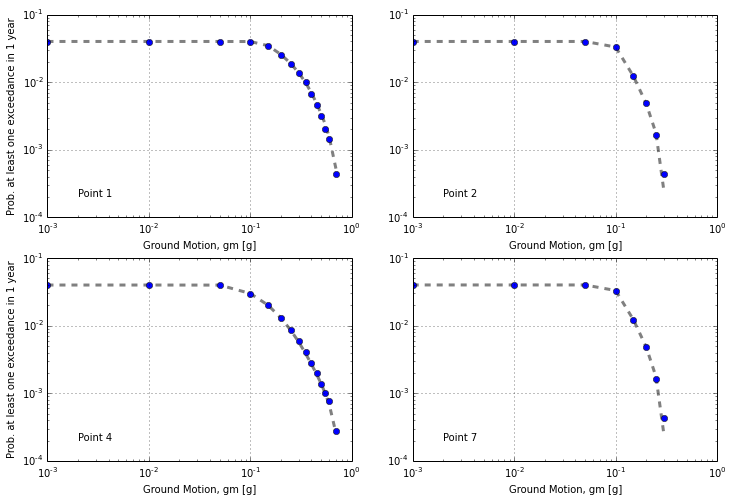
\includegraphics[width=14cm]{./Pictures/qa/test05_set1.png}
\caption{Comparison between the results provided by \textcite{thomas2010}
for the test case 5 set 1 (grey dashed lines) and the \gls{acr:oqhl} 
(green dots). The sites considered have the following indexes: 
1, 2, 3, 4 (see Figure \ref{fig:peer_sources})}
\label{fig:peer_set1_test5}
\end{figure}
% . . . . . . . . . . . . . . . . . . . . . . . . . . . . . . . . . . . < Figure
    %
    \clearpage
    \item [Test case 10]
        This test considers one uniform area source with a truncated exponential 
        model with $M_{min}$ of 5.0, $M_{max}$ 6.5, b-value of 0.9 and an annual 
        rate $M_W \geq M_{min}$ of 0.0395. As OpenQuake defines finite rupture 
        planes for each of the points considered in the area source, the scaling
        relation was fixed such that the area of the finite rupture was equal to 
        1.0 km. Hypocentral depth is fixed at 5 km. 
        %
        The preferred GMPE is \cite{sadigh1997} for rock, with sigma set to 0.0. 
        The expected values for the unit tests are those provided in the appendix 
        of \cite{thomas2010} (page A - 15), which represent the mean values of the 
        distribution of estimates from the software considered. 
        %
        As these are not solved by hand, the test are considered to pass when the 
        following condition is satisfied for all values:
        \begin{equation}
        |calculated - expected| \leq \left( {atol + rtol * |expected|} \right)
        \end{equation}
        where $atol$ and $rtol$ are the absolute and relative difference 
        between two terms, set to $10^{-4}$ and $10^{-1}$ respectively.
% . . . . . . . . . . . . . . . . . . . . . . . . . . . . . . . . . . . > Figure
\begin{figure}[!ht]
\centering
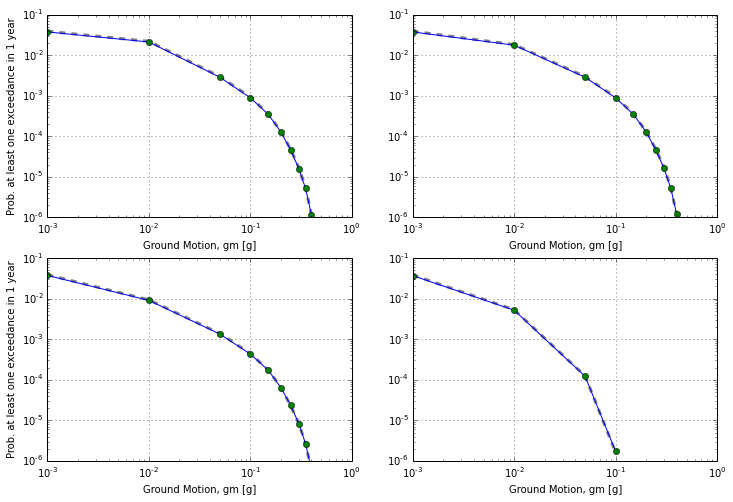
\includegraphics[width=14cm]{./Pictures/qa/test10_set1.png}
\caption{Comparison between the results provided by \textcite{thomas2010}
for the test case 10 set 1 (grey dashed lines) and the \gls{acr:oqhl} 
(green dots). The sites considered have the following indexes: 
1, 2, 3, 4 (see Figure \ref{fig:peer_sources}).}
\label{fig:peer_set1_test10}
\end{figure}
% . . . . . . . . . . . . . . . . . . . . . . . . . . . . . . . . . . . < Figure
    \clearpage
    \item [Test case 11]
        The same area source and GMPE are considered as for 
        \textbf{Set 1 Case 10}; 
        however, the hypocentral depth is distributed uniformly between 5 km 
        and 10 km. All other conditions are the same.
% . . . . . . . . . . . . . . . . . . . . . . . . . . . . . . . . . . . > Figure
\begin{figure}[!ht]
\centering
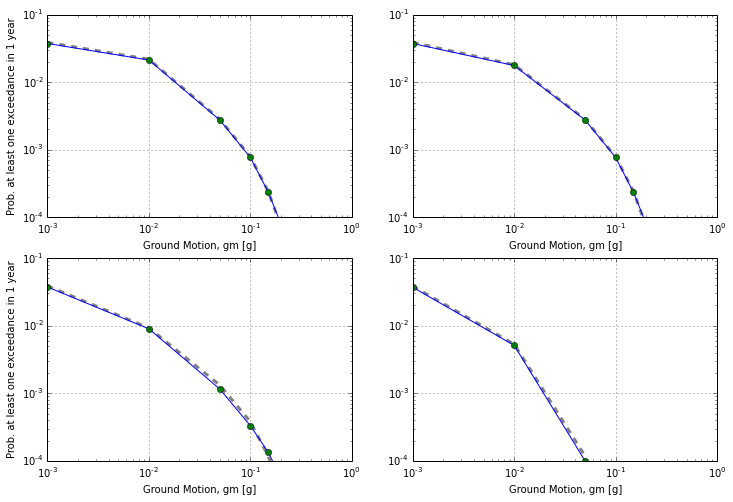
\includegraphics[width=14cm]{./Pictures/qa/test11_set1.png}
\caption{Comparison between the results provided by \textcite{thomas2010}
for the test case 11 set 1 (grey dashed lines) and the \gls{acr:oqhl} 
(green dots). The sites considered have the following indexes: 
1, 2, 3, 4 (see Figure \ref{fig:peer_sources}).}
\label{fig:peer_set1_test11}
\end{figure}
% . . . . . . . . . . . . . . . . . . . . . . . . . . . . . . . . . . . < Figure
\end{description}
